\documentclass[twocolumn,aps,pra,notitlepage,superscriptaddress,longbibliography,nofootinbib]{revtex4-1}
\usepackage{amsmath,amssymb,amsthm,mathtools,mathrsfs}
\usepackage[table,dvipsnames]{xcolor}%
\usepackage{tikz}
\usetikzlibrary{quantikz2}

\begin{document}

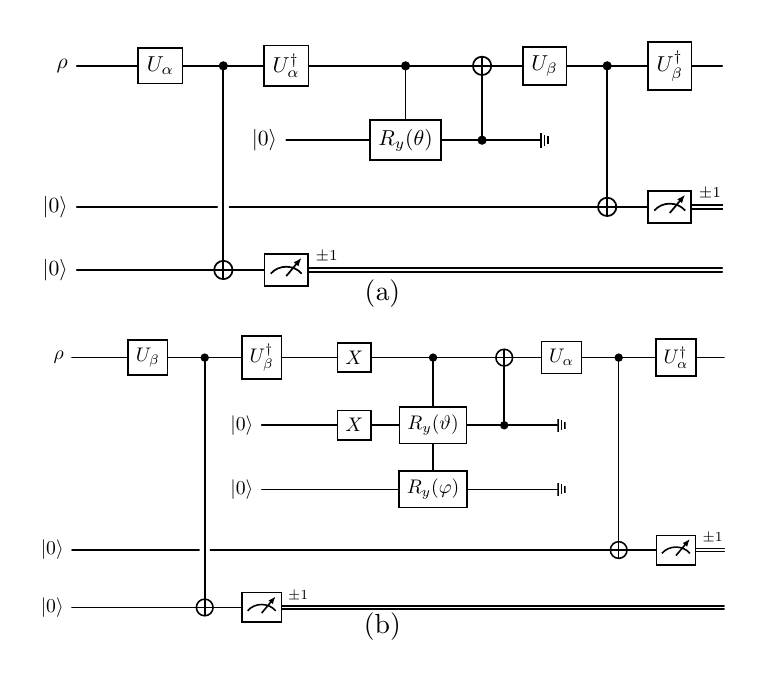
\begin{tikzpicture}
\node[scale=0.78] at (0,0) {
\begin{quantikz}
\setwiretype{n} & \lstick{$\rho$} & \setwiretype{q} & \gate{U_{\alpha}} & \ctrl{3} & \gate{U_{\alpha}^{\dag}} & & \ctrl{1} & \targ{} & \gate{U_{\beta}} & \ctrl{2} & \gate{U_{\beta}^{\dag}} & \\ 
\setwiretype{n}  & & & & & \lstick{\ket{0}} & \setwiretype{q} & \gate{R_{y}(\theta)} & \ctrl{-1} & \ground{} \\
\setwiretype{n} & \lstick{\ket{0}} & \setwiretype{q} & & \push{\phantom{x}} & & & & & & \targ{} & \meter{} & \setwiretype{c} \wire[l][1]["\pm 1"{above,pos=0.4}]{a} \\
\setwiretype{n} & \lstick{\ket{0}} & \setwiretype{q} & & \targ{}\wire[u][3]{q} & \meter{} & \setwiretype{c} \wire[l][1]["\pm 1"{above,pos=0.4}]{a} & & & & & &
\end{quantikz}
};
\node at (0,-1.65) {(a)};
\node[scale=0.71] at (0,-4) {
\begin{quantikz}
\setwiretype{n} & \lstick{$\rho$} & \setwiretype{q} & \gate{U_{\beta}} & \ctrl{3} & \gate{U_{\beta}^{\dag}} & & \gate{X} & \ctrl{2} & \targ{} & \gate{U_{\alpha}} & \ctrl{3} & \gate{U_{\alpha}^{\dag}} & \\ 
\setwiretype{n}  & & & & & \lstick{\ket{0}} & \setwiretype{q} & \gate{X} & \gate{R_{y}(\vartheta)} & \ctrl{-1} & \ground{} \\
\setwiretype{n}  & & & & & \lstick{\ket{0}} & \setwiretype{q} & & \gate{R_{y}(\varphi)} & & \ground{}  \\
\setwiretype{n} & \lstick{\ket{0}} & \setwiretype{q} & & \push{\phantom{x}} & & & & & & & \targ{} & \meter{} & \setwiretype{c} \wire[l][1]["\pm 1"{above,pos=0.4}]{a} \\
\setwiretype{n} & \lstick{\ket{0}} & \setwiretype{q} & & \targ{}\wire[u][3]{q} & \meter{} & \setwiretype{c} \wire[l][1]["\pm 1"{above,pos=0.4}]{a} & & & & & & &
\end{quantikz}
};
\node at (0,-5.875) {(b)};
\end{tikzpicture}

\end{document}